% ======================================================================================
% CLUSTERING
%
% graphs to insert:
%	- score vs silhouette coefficient per cluster
%	- sample silhouette values for the best number of clusters
%	- 3D/2D cluster representation for the best number of clusters
% tables to insert:
%	- PCA outcome of the features
%	- object to cluster assignment depending on number of clusters (the best ones)
%	- cluster sizes depending on number of clusters
% figures:
%	- mean values of the features per cluster applied to the object


\section{Clustering}

\subsection{PCA}

PCA was performed to keep the three most variant features of the samples. In \ref{tab:pca_components} we can see the principle axes for maximum variance in the data, and from there we can see that the features rotation, and direction are the most variant features. In \ref{tab:pca_variance} we can see the variance for each of these three features as well as their ratio for the dataset. In total these features represent around 80\% of the entire variance, seeing how we have five in total, this would mean that the other two would represent around 10\% each which is of quite small significance compared to the other three, we therefore can be quite happy about this new dimensional reduction.

\begin{table}
	\begin{tabular}{ c c c c c }
		\hline
		\multicolumn{5}{c}{Principal Components} \\ \hline
		-0.51661962 & -0.51137137 &  0.59560332 &  0.29608388 &  0.17086402 \\ \hline
		-0.36102909 &  0.33317829 & -0.15354445 & -0.22331964 &  0.82776969 \\ \hline
		-0.07275141 & -0.28151638 &  0.19427207 & -0.92743392 & -0.13259127 \\ \hline
	\end{tabular}
	\caption{Principal axes in feature space, representing the directions of maximum variance in the data.}
	\label{tab:pca_components}
\end{table}

\begin{table}
	\begin{center}
		\begin{tabular}{cc}
			\hline
			Variance & Ratio \\ \hline
			1.9754988 & 0.39498577 \\
			1.12242609 & 0.22442045 \\
			0.89518261 & 0.17898487 \\
			\hline
		\end{tabular}
		\caption{Variance and their ratio for the principal features.}
		\label{tab:pca_variance}
	\end{center}
\end{table}


\subsection{K-means}

K-means was later run on the transformed data for cluster numbers ranging two to fifteen. As to choose the best fit of number of clusters we later look at the mean silhouette coefficient and sum of squared distances from each sample to their closest cluster center. These results are presented in \ref{fig:kmeans_score}. By using the \texttt{elbow method} on the graph containing the sum of squared distances for the samples we can judge that a number of clusters between five and eight is suitable. With the help of the silhouette score, where six clusters gives the best results, and which falls into this range, we can conclude that six clusters is a good fit.

Figure \ref{fig:silhouette_coef} shows us the silhouette coefficient per sample for the three cases of five, six and seven clusters. We can see that for five clusters there are a lot of samples that have a very poor coefficient in some clusters. Seven has a better repartition but the gradient is quite important for the larger clusters. While six gives us something more balanced, and thus confirming it is a better choice.

Figure \ref{fig:clusters} show us a two-dimensional and three-dimensional representation of the data divided into clusters and their centers. It is not entirely obvious how the data is clustered as the data is a bit hard to reduce in dimensionality.

\begin{figure}
	\begin{subfigure}[b]{\textwidth}
		\input{plot_clustering__mean-silhouette}
		\caption{Mean silhouette coefficient per number of clusters.}
	\end{subfigure}
	\begin{subfigure}[b]{\textwidth}
		\input{plot_clustering__sum-sqr-dist}
		\caption{Sum of squared distances per sample to their closest cluster by number of clusters. Used in the \texttt{elbow method}.}
	\end{subfigure}
	\caption{Mean silhouette coefficient and sum of squared distances per sample to their closest cluster, depending on number of clusters. \texttt{best fit} identifies the possible best number of clusters in accordance to the maximum value of the mean silhouette coefficient and the elbow method.}
	\label{fig:kmeans_score}
\end{figure}

\begin{figure}
	\begin{subfigure}[b]{\textwidth}
		\input{plot_silhouette_5}
		\caption{Silhouette coefficient per samples for five clusters.}
	\end{subfigure}
	\begin{subfigure}[b]{\textwidth}
		\input{plot_silhouette_6}
		\caption{Silhouette coefficient per samples for six clusters.}
	\end{subfigure}
\end{figure}
\begin{figure}
	\ContinuedFloat
	\begin{subfigure}[b]{\textwidth}
		\input{plot_silhouette_7}
		\caption{Silhouette coefficient per samples for seven clusters.}
	\end{subfigure}
	\caption{Silhouette coefficient per sample in each cluster for five, six and seven number of clusters.}
	\label{fig:silhouette_coef}
\end{figure}

\begin{figure}
	\begin{subfigure}[b]{\textwidth}
		\input{plot_clustering__clusters-2d}
		\caption{Two-dimensional representation of the samples and their assigned clusters and centroids.}
	\end{subfigure}
	\begin{subfigure}[b]{\textwidth}
		\input{plot_clustering__clusters-3d}
		\caption{Three-dimensional representation of the samples and their assigned clusters and centroids.}
	\end{subfigure}
	\caption{A two-dimensional and three-dimensional representation of the sample space with their assigned clusters and centroids for six clusters.}
	\label{fig:clusters}
\end{figure}


\subsection{Object cluster assignments}

\begin{figure}
	\input{plot_clustering__obj-sampl-assgmnt}
	\caption{}
\end{figure}

\begin{table}
	\begin{tabular}{|c|l|}
		\hline
		Cluster & Objects \\
		\hline
		one   & hammer, pen, scalpell, scissors, knife, screwdriver, brush \\
		two   & tube \\
		three & can, pitcher, glass, bottle, cup \\
		four  & box \\
		five  & cutters \\
		six   & - \\
		\hline
	\end{tabular}
	\caption{Cluster assignment of objects between six clusters.}
	\label{tab:object_cluster_assign}
\end{table}


% TODO create images of the objects with the mean values of their cluster on them
%\begin{figure}
	%\centering
	%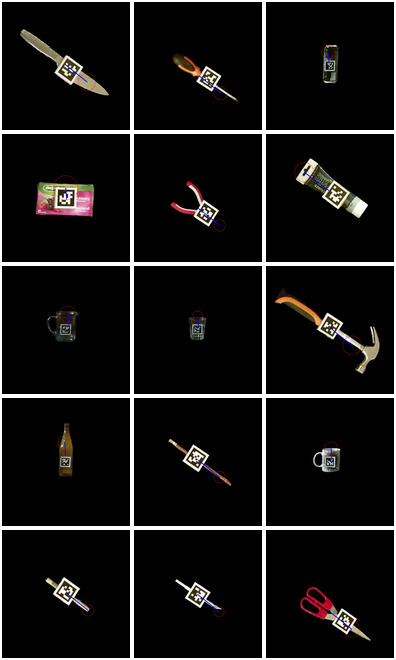
\includegraphics[width=\textwidth]{img/results/object_handovers.jpg}
	%\caption{Resulting handover data applied to each object}
	%\label{fig:object_handovers}
%\end{figure}



% ======================================================================================
% CLASSIFICATION
%
% GRAPHS:
%	- loss per step
%	- accuracy per step (validation and testing)
%	- training speed
% TABLES:
%	- confusion matrix
%	- accuracy per object
%	-

\section{Classification}
Output different results from classification depending on which layers are trained further and network architecture.

\subsection{Initial testing of batch sizes and learning rates}

\subsubsection{Learning rates}

\begin{figure}
	\begin{subfigure}[b]{\textwidth}
		\input{plot_classification__learning-rates__loss}
		\caption{Loss.}
	\end{subfigure}

	\begin{subfigure}[b]{\textwidth}
		\input{plot_classification__learning-rates__val-acc}
		\caption{Validation accuracy.}
	\end{subfigure}
\end{figure}

\begin{figure}
	\ContinuedFloat
	\begin{subfigure}[b]{\textwidth}
		\input{plot_classification__learning-rates__test-acc}
		\caption{Test accuracy.}
	\end{subfigure}
	\caption{Loss, validation and test accuracy for batch size 32 and different learning rates.}
\end{figure}


\subsubsection{Batch sizes}

\begin{figure}
	\begin{subfigure}[b]{\textwidth}
		\input{plot_classification__batch-sizes__loss}
		\caption{Loss.}
	\end{subfigure}

	\begin{subfigure}[b]{\textwidth}
		\input{plot_classification__batch-sizes__val-acc}
		\caption{Validation accuracy.}
	\end{subfigure}
\end{figure}

\begin{figure}
	\ContinuedFloat
	\begin{subfigure}[b]{\textwidth}
		\input{plot_classification__batch-sizes__test-acc}
		\caption{Test accuracy.}
	\end{subfigure}
	\caption{Loss, validation and test accuracy for learning rate 1e-05 and different batch sizes.}
\end{figure}


\subsection{Finetuning parameters}

\subsection{End results}

\begin{figure}
	\input{plot_classification__confmat}
	\caption{Confusion matrix.}
\end{figure}
